% Copyright 2004 by Till Tantau <tantau@users.sourceforge.net>.
%
% In principle, this file can be redistributed and/or modified under
% the terms of the GNU Public License, version 2.
%
% However, this file is supposed to be a template to be modified
% for your own needs. For this reason, if you use this file as a
% template and not specifically distribute it as part of a another
% package/program, I grant the extra permission to freely copy and
% modify this file as you see fit and even to delete this copyright
% notice. 
\usepackage{graphicx}

\documentclass{beamer}
\usepackage{graphicx}
\usepackage[table]{xcolor}
\usepackage{color, colortbl}
\usepackage{subfig}
\definecolor{blue}{rgb}{0, 0, 255}

% There are many different themes available for Beamer. A comprehensive
% list with examples is given here:
% http://deic.uab.es/~iblanes/beamer_gallery/index_by_theme.html
% You can uncomment the themes below if you would like to use a different
% one:
%\usetheme{AnnArbor}
%\usetheme{Antibes}
%\usetheme{Bergen}
%\usetheme{Berkeley}
%\usetheme{Berlin}
%\usetheme{Boadilla}
%\usetheme{boxes}
%\usetheme{CambridgeUS}
%\usetheme{Copenhagen}
%\usetheme{Darmstadt}
%\usetheme{default}
%\usetheme{Frankfurt}
%\usetheme{Goettingen}
%\usetheme{Hannover}
\usetheme{Ilmenau}
%\usetheme{JuanLesPins}
%\usetheme{Luebeck}
%\usetheme{Madrid}
%\usetheme{Malmoe}
%\usetheme{Marburg}
%\usetheme{Montpellier}
%\usetheme{PaloAlto}
%\usetheme{Pittsburgh}
%\usetheme{Rochester}
%\usetheme{Singapore}
%\usetheme{Szeged}
%\usetheme{Warsaw}

\title{PageRank Algorithm : Multithreading Vs GraphX Spark Implementation}

% A subtitle is optional and this may be deleted
\subtitle{CS-527 Parallel Computer Architectures}

\author{Jack Kolokasis}
% - Use the \inst{?} command only if the authors have different affiliation.

\institute[kolokasis@csd.forth.gr] % (optional, but mostly needed
% - Use the \inst command only if there are several affiliations.
% - Keep it simple, no one is interested in your street address.

\date{\today}
% - Either use conference name or its abbreviation.
% - Not really informative to the audience, more for people (including yourself)
%   who are reading the slides online

% This is only inserted into the PDF information catalog. Can be left out. 

% If you have a file called "university-logo-filename.xxx", where xxx is a
% graphic format that can be processed by latex or pdflatex, resp., then you can
% add a logo as follows:

 \pgfdeclareimage[height=1.5cm]{university-logo}{UoC_logo.png}
 \titlegraphic{\pgfuseimage{university-logo}\hspace*{-7.75cm}~% 
 }

% Delete this, if you do not want the table of contents to pop up at the
% beginning of each subsection:

%\AtBeginSection[]
%{
%  \begin{frame}<beamer>{Outline}
%    \tableofcontents[currentsection,currentsubsection]
%  \end{frame}
%}

% Let's get started
\begin{document}

\begin{frame}
  \titlepage
\end{frame}

\begin{frame}{Outline}
    \tableofcontents
  % You might wish to add the option [pausesections]
\end{frame}

\section{Motivation \& Overview}

\begin{frame}{PageRank Is Fun}
    \begin{figure}
        
\includegraphics[width=8cm, height=5cm]{figure1.png}
    \end{figure}

    \begin{itemize}
            %toDo
            % Formatting the text here
            %
            PageRank if fun \\
            .... but there are a LOT of Pages with a LOT of Links
            and it becomes a LOT of work to calculate.
    \end{itemize}

\end{frame}

\begin{frame}{Overview}{How Does PageRank Work}
    \begin{minipage}{4cm}
        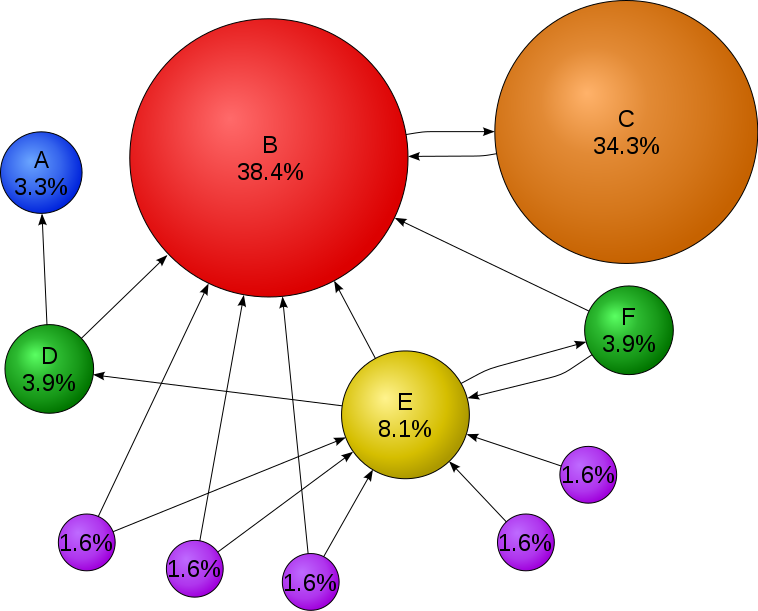
\includegraphics[height=4cm, width=4cm]{figure2.png}
    \end{minipage}%
    \begin{minipage}{7cm}
        \begin{itemize}
            \item{Directed Graph}
                
                (nodes point to other nodes but it's one way
                street)
            \item{Initialize all the node with a default probability: 
                $$PR(p_i;0) = \frac{1}{N}$$
                }
            \item{For every node in the graph calculate a rank on every iteration: 
                $$PR(p_i;{t+1}) = \frac{1-d}{N} + d\sum_{p_j\in
                M(p_i)}\frac{PR(p_j)}{out(p_j)}$$ }
        \end{itemize}
    \end{minipage}
\end{frame}

\section{Multithreading Implementation}
\begin{frame}{Multithreading Implementation}{Read Input Datase and Construct the
    Graph}
    \begin{figure}
        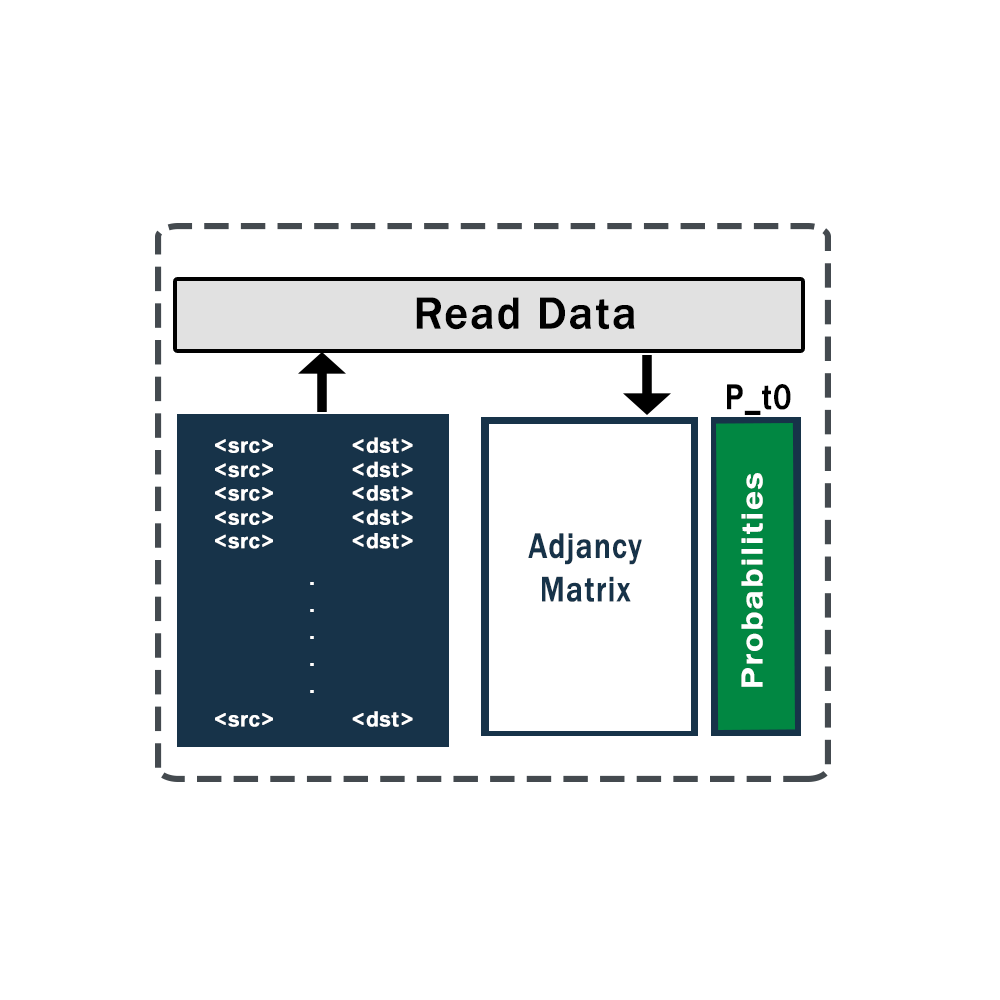
\includegraphics[width=8cm, height=6cm]{implementation1.png}
    \end{figure}
\end{frame}

\begin{frame}{Multithreading Implementation}{Computation of PageRank Algorithm}
    \begin{figure}
        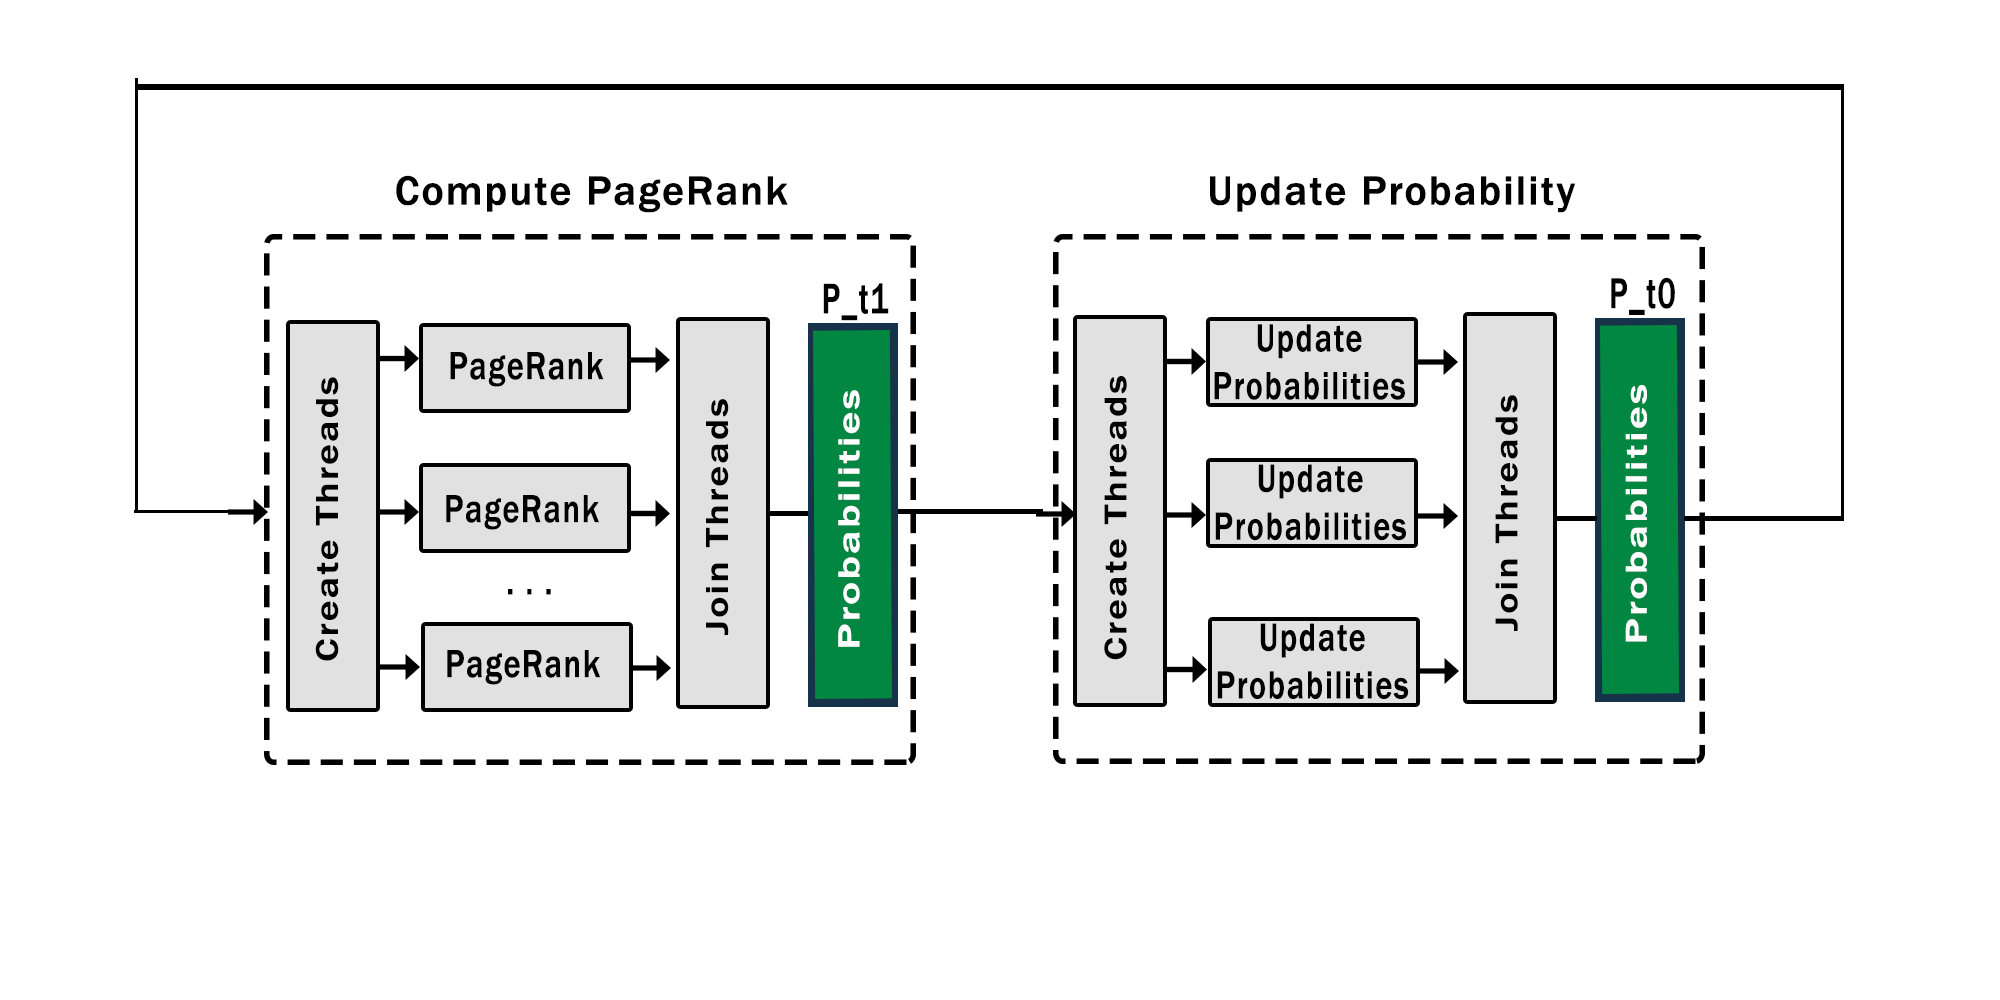
\includegraphics[width=10cm, height=6cm]{implementation2.png}
    \end{figure}
\end{frame}

\section{GraphX Spark Implementation}
\begin{frame}
\end{frame}

\section{Evaluation & Results}
\begin{frame}{Evaluation}
    \begin{itemize}
        \item{Compare Computation Time of PageRank Multithreading against Spark
            GraphX Pagerank Implementation executing on single node}
            \begin{itemize} 
                \item{Machine Specifications:}
                    \begin{itemize}
                        \item{\textbf{CPU:} Intel(R) Xeon(R) CPU E5-2630 V3 @ 2.40GHz} 
                        \item{\textbf{Number of Cores:} 32 cores}
                        \item{\textbf{Memmory Size:} 256GB}
                        \item{\textbf{OS:} CentOS Linux \textbf{Version:} 7 (Core)}
                    \end{itemize}

                \item{Multithreading Pagerank}
                    \begin{itemize}
                        \item{Use 1, 2, 4, 8, 16, 32 number of threads
                    respectively.}
                    \end{itemize}
            \end{itemize}
    \end{itemize}

\end{frame}

\begin{frame}{Evaluation}
    \begin{itemize}
            \begin{itemize}
                \item{Spark GraphX Pagerank}
                    \begin{itemize}
                        \item{1 executor: 1, 2, 4 ,8, 16, 32 cores respectively}
                        \item{Different number of executors :}
                            \begin{itemize}
                                \item{1 executor: 32 cores and 125GB memory}
                                \item{2 executor: 16 cores and 125GB memory}
                                \item{4 executor: 8 cores and 60GB memory}
                                \item{8 executor: 4 cores and 30GB memory}
                                \item{16 executor: 2 cores and 15GB memory}
                                \item{32 executor: 1 cores and 7GB memory}
                            \end{itemize}
                    \end{itemize}

                \item{Average of 5 runs}

                \item{Graphs Datasets}
                    \begin{table}
                        \centering
                        \begin{tabular}{|l|c|c|c|}
                            \hline
                            \rowcolor{blue} 
                            \color{white}\textbf{Dataset} &\color{white}
                            \textbf{Vertex} &\color{white} \textbf{Edges} \\
                            \hline
                            Dataset1   &10,000   &1,000,000 \\
                            \hline
                            Dataset2  &10,000  &10,000,000 \\
                            \hline
                            Dataset3   &100,000  &20,000,000 \\
                            \hline
                        \end{tabular}
                    \end{table}


            \end{itemize}
    \end{itemize}
\end{frame}
\section{Conclusions}

\begin{frame}


\end{frame}

%\item{Testing Multithreaded PageRank execution using 1, 2, 4, 8,
%                    16, 32 number of threads respectively.}
%                \item{Testing Spark GraphX Pagerank implementations using 1
%                    executor with 1,2,4,8,16,32 cores respectively.}
%                \item{Testing Spark GraphX Pagerank implementations:}
%                    \begin{itemize}
%                        \item{1 executor: 1, 2, 4 ,8, 16, 32 cores respectively}
%                        \item{1 executor: 32 cores, 2 executors: 16 cores each,
%                            4 executors: 8 cores each, 16 executors: 2 cores
%                            each and 32 executors: 1 core each}
%
\end{document}
